\chapter{基于STRIDE对车载IVI系统的威胁建模}
\label{ch3}
本章首先介绍了基于STRIDE的威胁建模过程并说明车载IVI系统所面临的潜在风险和安全威胁, 最后基于STRIDE威胁模型对一个车载系统进行实例威胁分析和威胁评级。

\section{IVI系统基本功能架构}
IVI系统是一种嵌入式系统,一般由硬件和软件两部分组成。开发IVI系统需要进行需求分析、系统架构设计、硬件设计、软件开发、测试和调试等多个环节。其中,需求分析和系统架构设计是IVI系统开发的重要基础,硬件设计和软件开发是IVI系统开发的核心步骤,测试和调试是确保IVI系统质量的关键环节。整个IVI系统的开发需要团队协作,综合考虑到硬件和软件两方面,以提供高性能、稳定性和易用性的IVI系统。
一些著名的汽车IVI系统的具体情况如表 3.1 所示
\begin{table}[h]
  \centering
  \begin{tabular}{@{}lll@{}}
      \toprule
      厂商 & 系统名称 & 车型 \\
      \midrule
      丰田 & Entune & 多款车型 \\
      本田 & HondaLink & 多款车型 \\
      日产 & NissanConnect & 多款车型 \\
      福特 & SYNC & 多款车型 \\
      雪佛兰 & Chevy MyLink & 多款车型 \\
      捷豹路虎 & InControl & 多款车型 \\
      宝马 & iDrive & 多款车型 \\
      奥迪 & MMI & 多款车型 \\
      梅赛德斯-奔驰 & COMAND & 多款车型 \\
      \bottomrule
  \end{tabular}
  \caption{常用汽车厂商的IVI系统}
\end{table}
为了有目的地进行 IVI系统的网络安全性风险的研究,本文从基础的角度,结合各种车辆的 IVI系统的基础设施和功能,从理论上总结出 IVI的基本功能架构。
IVI的基础功能体系结构包括应用、通讯、控制、控制等模块。

通讯模组因车辆配置 IVI的内容及模式而异,在车辆网络中,一般包含4 G/5 G、蓝牙、 Wi-Fi、 DSRC等通讯手段,也有一些车辆连接 GPS、G-Sensor、V-Sensor等位置及局部感应装置,另外,通讯模组还设有 USB、 SD等外接装置,也可通过T-BOX与外界终端进行通讯。IVI系统通过通信模块所实现的有线无线通信方式,与诸如 TSP、智能终端、智能网联车辆等的车辆外设备进行通信,包括数据、短信、语音等。如图3.1 所示 我们给出了IVI系统的基本功能结构。
\begin{figure}
  \centering
  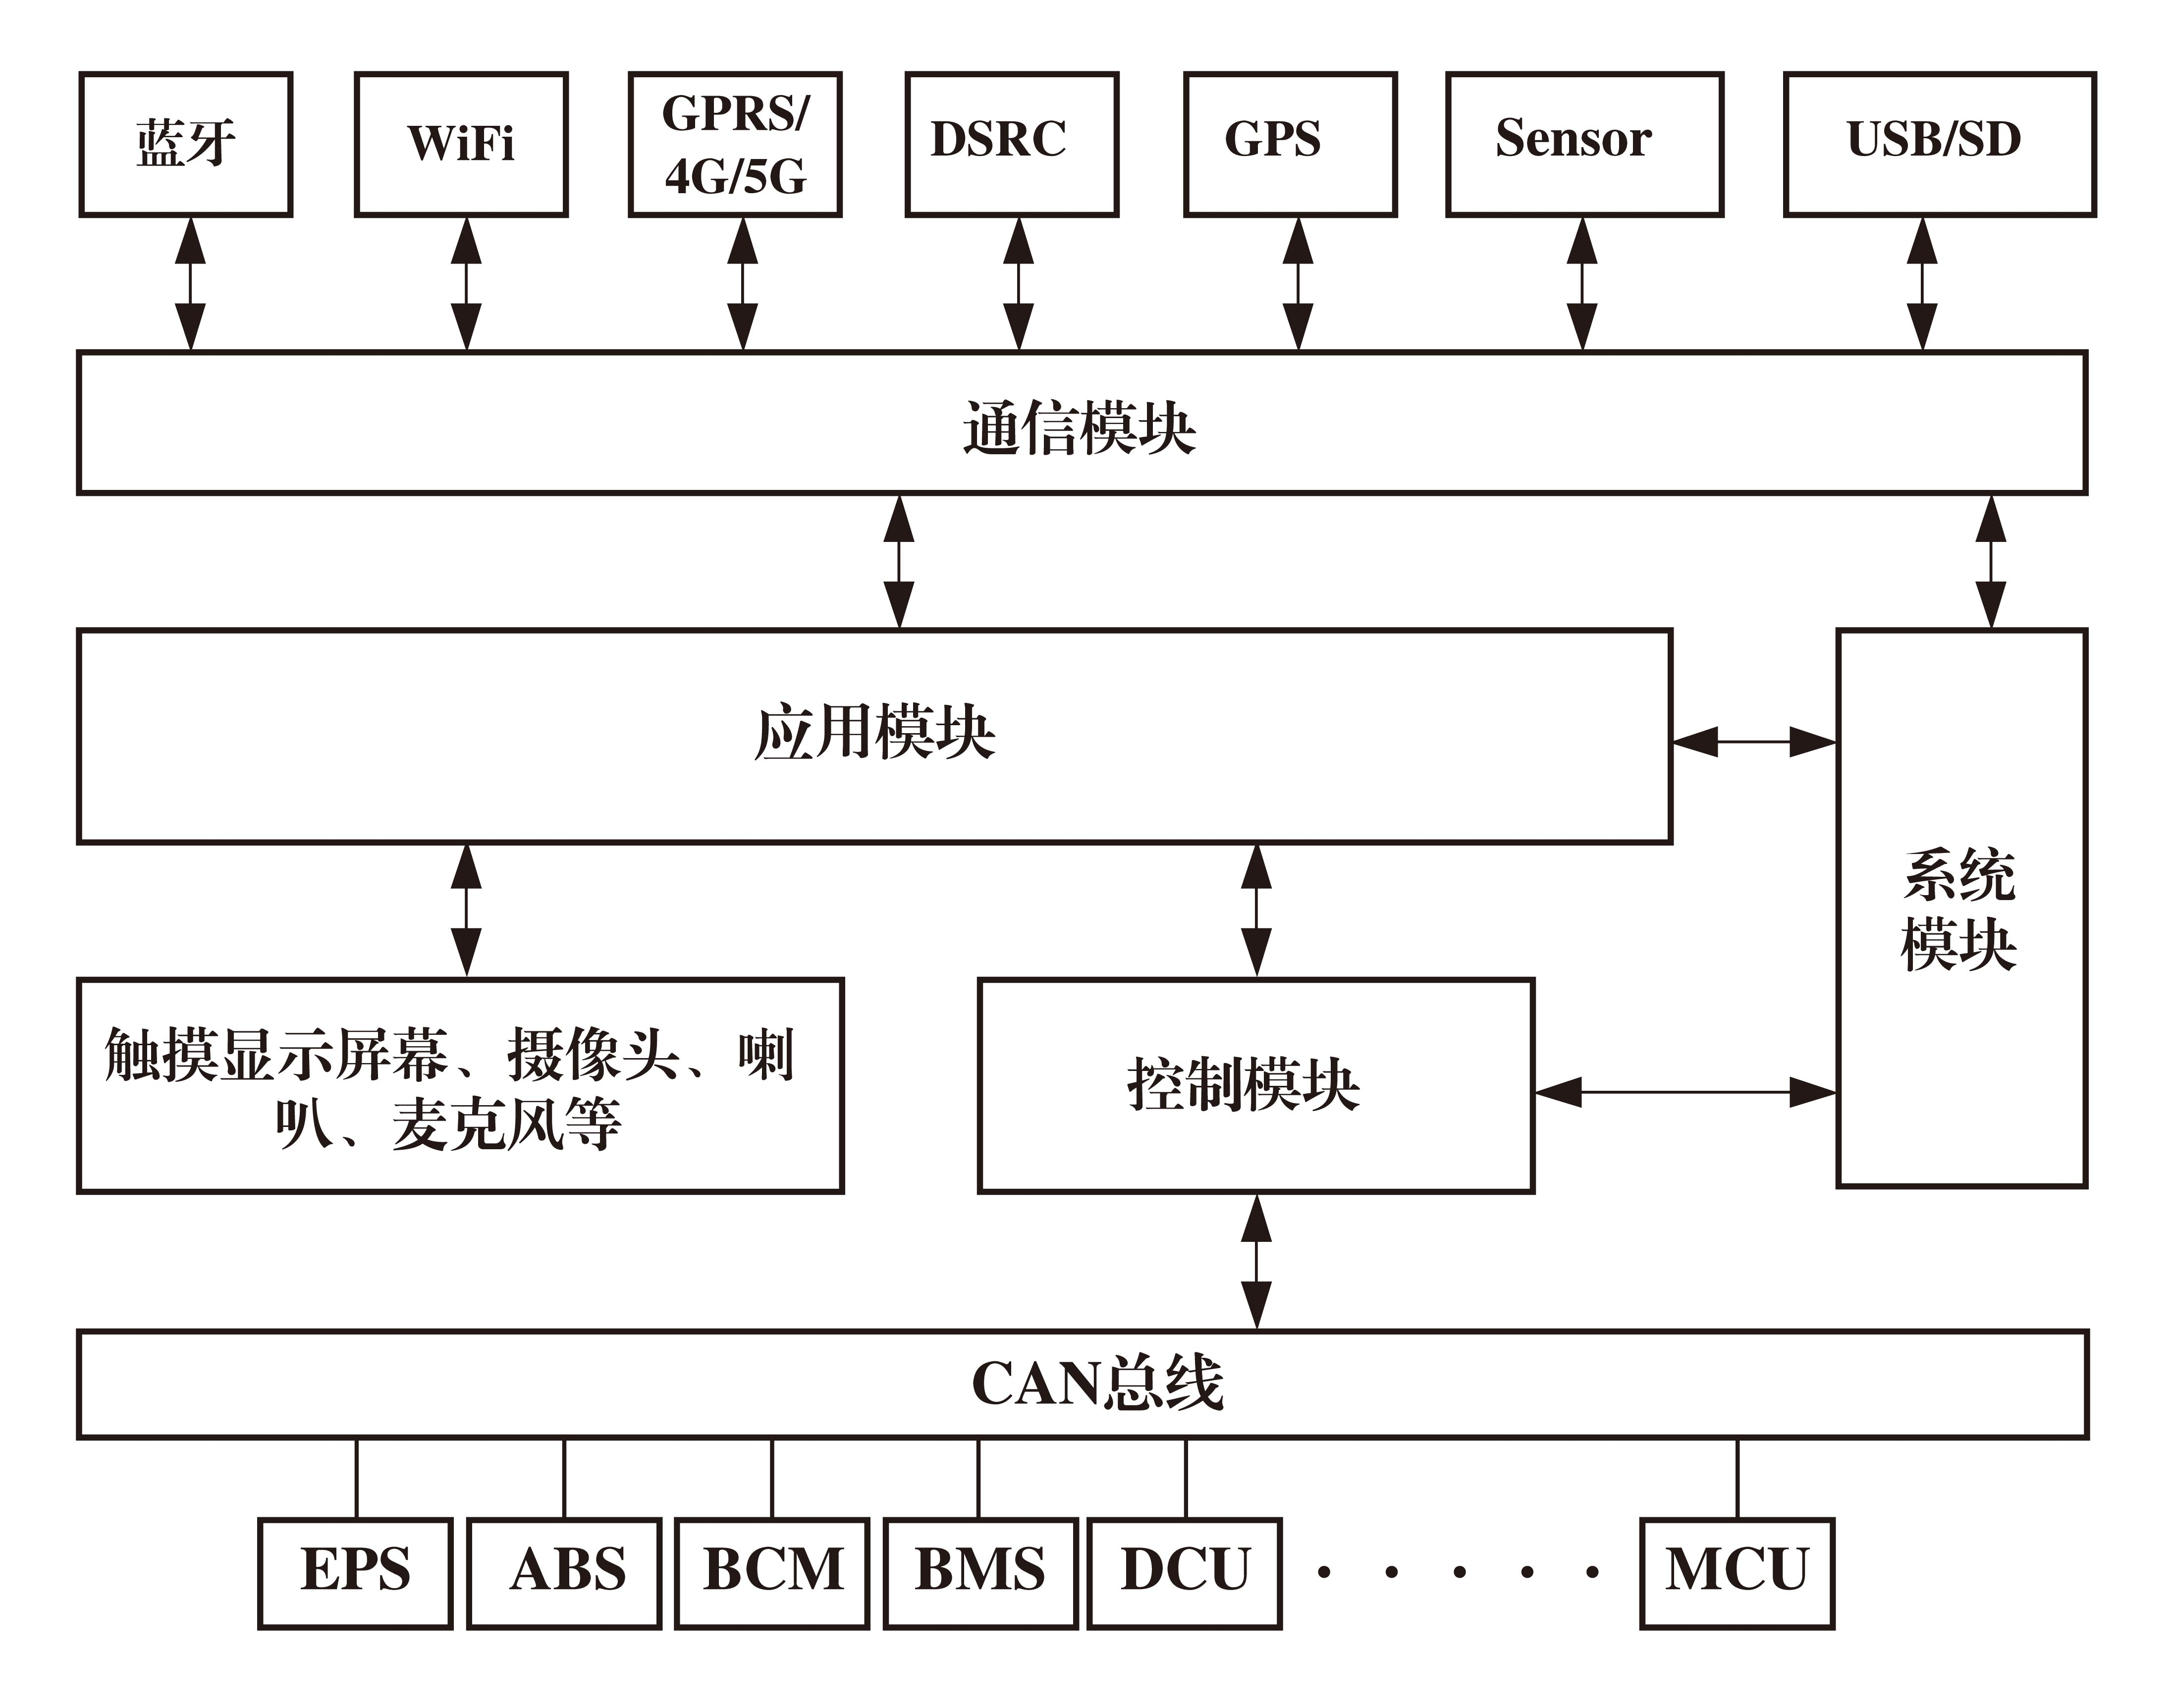
\includegraphics[scale=0.4]{resources/img/a50.jpg}
  \caption{IVI系统基础模块结构}
\end{figure}
IVI系统的基本功能架构由多个部分组成,下面详细说明:

主机部分:主机是IVI的核心部分,包括处理器、内存、存储器、接口等。处理器用于处理IVI系统的各种计算任务,内存用于存储IVI系统的运行数据,存储器用于存储IVI系统的程序和数据,接口用于连接其他设备和传输数据。

显示器部分:显示器用于显示IVI系统的图形用户界面和相关信息。IVI系统的显示器一般采用触摸屏或非触摸屏两种形式,可以显示多媒体内容、导航地图、车辆状态等信息。

输入设备部分:输入设备用于用户输入信息,可以是触摸屏、物理按键、语音识别等。通过输入设备,用户可以控制IVI系统的各种功能,例如切换音乐、调整空调等。

音频系统部分:音频系统用于处理IVI系统的音频信息,包括音频解码器、放大器、扬声器、麦克风等。通过音频系统,用户可以听取音乐、电话、导航语音等信息。

网络连接部分:网络连接用于连接IVI系统和外部网络,包括蓝牙、Wi-Fi、GPS等。通过网络连接,IVI系统可以与外部设备进行数据交换和通信,例如手机、互联网、车载系统等。

应用程序部分:应用程序是IVI系统的具体功能和服务,包括导航、娱乐、通讯等。应用程序可以通过显示器和输入设备进行交互,提供各种功能和服务。

总的来说,IVI系统的基本功能架构需要考虑到硬件和软件两方面,以确保系统的性能和稳定性。主机和显示器是IVI系统的核心部分,输入设备和音频系统是提供良好用户体验的重要组成部分,网络连接和应用程序则是IVI系统与外部世界进行交互和提供具体服务的关键。
\section{IVI系统的安全风险分析}
通过对 IVI系统外部网络环境、内部网络结构、应用运行平台、业务功能服务等方面的分析,认为 IVI网络的安全性因素主要有:外部通信实体、无线通信网络、车载物理设备、 IVI操作系统、 IVI应用服务、 IVI应用数据、车载总线网络等。

\subsection{外部通信实体安全风险}

IVI系统的外部通信主体包括用户、外部设备、车辆总线、云服务和第三方应用程序。作为最终使用者,用户通过触摸屏、物理按键、语音控制等方式与IVI系统进行交互,从而实现对车载娱乐、导航、通讯等功能的使用。外部设备是IVI系统的扩展,通过蓝牙、USB等通信协议与IVI系统连接,实现多媒体、导航等功能的互通。车辆总线是连接车内各个电子设备的数据总线,IVI系统需要与车辆总线进行通信,才能获取车辆的状态信息,以及控制车内其他电子设备。通过互联网连接云端的气象和交通数据服务,获取当前位置的天气和路况等信息。另外,IVI系统可以支持第三方应用程序,这些应用程序通过与IVI系统进行交互,实现在车内使用的功能。

\subsection{无线通信网络安全风险}

IVI系统作为一个复杂的系统,集成了多个功能模块,包括GPS导航、蓝牙连接和Wi-Fi接入等。这些模块都存在着潜在的漏洞和安全隐患,可能会被黑客利用。例如,黑客可能会通过蓝牙连接获取用户的个人信息,或者通过Wi-Fi接入控制车辆的功能等。如果黑客成功攻击了IVI系统,他们可能会窃取车主的个人信息,例如登录名、密码、信用卡信息等。这不仅会损害车主的个人隐私,也可能导致身份盗窃和金融欺诈等问题。
如果黑客能够远程控制IVI系统,他们可能会控制车辆的功能,例如加速、刹车、转向等,从而导致车辆失控,可能会引发交通事故。无线通信可能使得IVI系统感染病毒。例如,黑客可以通过无线网络向IVI系统传输病毒,导致系统崩溃或者失去控制。IVI系统中的蓝牙连接可能受到攻击,例如蓝牙拦截、蓝牙干扰等。黑客可以通过这些攻击方式获取用户的信息、窃取车辆的控制权或者干扰系统的正常工作。IVI系统中的Wi-Fi连接也可能受到攻击。例如,黑客可以利用恶意Wi-Fi网络欺骗用户连接假的Wi-Fi热点,并获取用户的敏感信息。


\subsection{IVI 操作系统安全风险} 

常用的IVI系统操作系统包括Android Auto、Apple CarPlay、QNX、Linux和Windows Embedded Automotive,这些操作系统旨在提供更好的用户体验、高度安全、可靠和灵活的车载娱乐和信息娱乐解决方案。不同的车辆制造商可能会使用不同的操作系统,或者选择自己开发或基于其他操作系统进行修改。

系统越狱风险   

汽车IVI系统越狱是指通过修改或绕过汽车娱乐信息系统的限制,获取超出正常用户权限的访问权限,以获取更多功能或控制汽车操作系统的行为。

(a) 系统稳定性降低。系统的越狱会对系统的稳定产生一定的干扰,从而提高系统死机、应用程序闪退、程序故障等问题。

(b) 安全机制失效。越狱可能会导致车载IVI系统的操作系统或应用程序被篡改,从而使原本的安全机制失效。例如,黑客可以通过越狱后安装的恶意软件来窃取车主的个人信息,这些软件可以绕过原有的数据加密和访问控制机制,直接获取数据。

(c) 系统固件升级问题。越狱后的系统可能会失去原有的安全保护机制,这使得黑客可以更轻松地利用系统漏洞进行攻击。而固件升级时,可能需要下载并安装未知来源的软件,这可能会增加系统受到攻击的风险。

IVI 应用服务安全风险 

IVI软件的安全性是指在 IVI基础上,在 IVI基础上的所有应用软件的安全。随着汽车网络的服务能力的发展,汽车上的各种应用软件都具备了网络的能力。这类软件是针对智能联网车辆进行远程打击的主要手段。

(1) 应用程序漏洞风险 

应用程序可能存在输入验证不充分的漏洞,这种漏洞可能会被黑客利用,通过输入恶意数据或代码来攻击IVI系统。SQL注入攻击、跨站点脚本攻击等类型的攻击都可以利用应用程序中的输入验证漏洞。
身份验证不安全也是应用程序常见的漏洞之一,比如密码弱或明文存储等,这会使黑客轻易地获取用户的身份认证信息,并获得对IVI系统的访问权限。
另外,应用程序可能存在缓冲区溢出漏洞,这种漏洞可能会被黑客利用,将恶意代码插入到应用程序的缓冲区中,从而实施攻击。
最后,应用程序在IVI系统中可能会存储敏感信息,如用户的登录凭据、个人资料等,如果这些数据没有得到妥善加密或保护,黑客就可以轻易地窃取这些信息。

(2)软件篡改风险 

篡改安卓应用程序可能会带来多种安全风险。其中最常见的是恶意代码注入。黑客可能会将恶意代码注入被篡改的应用程序中,导致应用程序在用户设备上执行恶意操作。例如,恶意代码可能会窃取用户的敏感信息,如个人身份信息、银行账户信息等,然后将这些信息发送到黑客的服务器上,从而导致用户的隐私泄露。此外,恶意代码还可能会感染用户设备病毒,导致设备功能异常、数据丢失等问题。
另一个安全风险是数据窃取。被篡改的应用程序可能会收集用户的敏感信息,然后将这些信息发送到黑客的服务器上,从而导致用户的隐私泄露。例如,黑客可能会窃取用户的个人身份信息、银行账户信息等,从而实施欺诈或其他形式的攻击。
篡改的应用程序还可能包含病毒。当用户安装这些应用程序时,病毒会感染用户的设备,导致设备功能异常、数据丢失等问题。此外,黑客还可能利用篡改的应用程序作为入口攻击用户设备或其他系统,进而造成更大的安全威胁。

\subsection{IVI 应用数据安全风险}

IVI系统一般包括车身控制,辅助驾驶,故障检测,导航定位,交通信息,移动办公,无线通讯,在线娱乐和 TSP等应用程序,其中包括汽车运行数据、汽车车主信息、汽车定位信息、车载应用系统数据等。IVI系统漏洞,应用程序漏洞,病毒和黑客入侵都会导致 IVI系统应用程序的资料遭到篡改、破坏、删除等行为,一些不经许可的应用程序和使用者可以存取一些机密资料,从而导致机密资料泄露。IVI系统的数据处理存在如下的安全性问题。
(a)外部安全威胁。而在 IVI系统中,黑客则通过 IVI系统漏洞、 IVI软件漏洞以及自身的安全漏洞来对 IVI系统数据、业务数据或数据库进行攻击。在系统的外部安全性方面,有未授权的应用,未授权的用户,未授权的数据访问,数据库通信协议的漏洞,系统平台的漏洞,认证的漏洞。 
(b) 内部安全威胁。如果使用者不小心存取机密资料,或不小心更改或移除资讯或使用者为未经许可之备份,则可能造成安全性危险。
(c) 共享数据。IVI操作系统、核心应用程序、通用应用程序共享的数据存贮器、共享共享、共享共享等多种形式的文件,导致了对系统和核心重要信息的恶意入侵;系统数据和隐私数据的明文保存也存在着数据泄漏的安全性问题。
(d) 非授权数据访问:应用程序可能会允许未经授权的用户访问应用程序数据,导致数据泄露和安全威胁。 

\subsection{车载物理设备安全风险}

IVI系统连接到互联网,因此黑客可以通过网络入侵车辆,从而控制车辆的物理设备,如发动机、转向和制动系统。这可能导致意外事故或车辆失控。IVI系统可能被病毒感染,这可能会导致IVI系统崩溃或停止工作。这可能会影响车辆的其他系统,如车载电子控制模块(ECM),从而导致车辆失控。IVI系统可能受到物理攻击,如破坏或意外碰撞。这可能导致IVI系统停止工作或影响车辆的其他系统。

\section{基于STRIDE的IVI威胁建模实例}
由于在第四章提出的威胁建模风险评估模型是结合了STRIDE建模方法, 因此本节将通过STRIDE模型对智能网联汽车车载娱乐系统IVI进行威胁建模,并以此为例对此进行风险评估
为后续的新型风险评估模型进行前置理论基础。

我们从内部环境和外部环境视角,对 IVI系统的攻击面和安全威胁进行了全面分析。
在此基础上,建立了 IVI系统的安全威胁建模模型如图3.2。
在 IVI 安全威胁方框模型中,以虚线为代表,上层为框图。
其中,最小的是外部实体,最小的是在方框图模型的底部。
在进行通讯时,通过的信任边界数目越多,其所面临的安全性风险也就越大。

\subsection{车载IIVI系统的STRIDE威胁模型}
威胁识别是通过构建STRIDE威胁建模来分析每条数据流及其关联资产是否容易受到S类、T类、R类、I类、D类和E类威胁,并对这些威胁进行识别和记录,从而对信息系统划分的各个数据流进行分析。如图3.2所示为STRIDE方法对IVI系统的威胁建模。
\begin{figure}
  \centering
  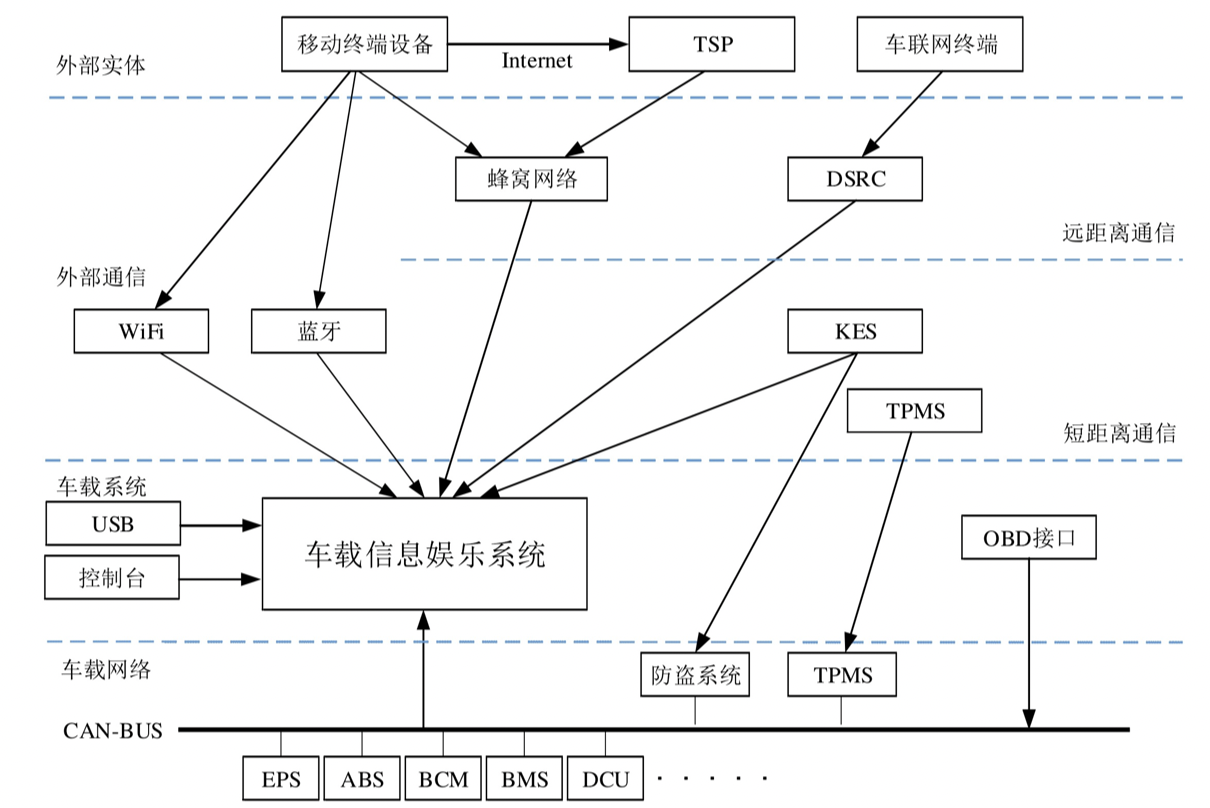
\includegraphics[scale=0.6]{resources/img/i33.png}
  \caption{车载娱乐IVI系统安全威胁建模图}
\end{figure}
\subsection{DF数据流威胁描述}
这里我们对三个外部元素:Wi-Fi, USB, GPS 进行威胁评级描述分析
并把它们的数据流分别称为: DF1, DF2, DF3。

(1)DF1 Wi-Fi与智能网联汽车IVI车载娱乐系统交互
该数据流可能面临的威胁有:攻击者通过劫持路由器伪装Wi-Fi信号, 窃听用户传输信息\cite{berghel2005Wi-Fi}

(2)DF2 USB与智能网联汽车IVI车载娱乐系统交互
该数据流可能面临的威胁有:通过USB设备的固件进行重新编程,来执行恶意行为,比如恶意文件下载、数据泄露等\cite{nissim2017usb}。

(3)DF2 GPS与智能网联汽车IVI车载娱乐系统交互
该数据流可能面临的威胁有:通过对搭载GPS传感器的车载信号接收器发送虚假信号, 从而误导汽车导航定位等\cite{alamleh2020cheat}。
\subsection{威胁评级和风险评估}
我们通过CVSS 通用漏洞评分系统对智能网联汽车来进行某个场景的漏洞评分和风险评估,在未经身份验证的情况下,攻击者可以远程接管汽车控制系统实现远程控制并可能造成交通事故等重大危害,我们对通过Wi-Fi这条攻击路径可以进行如下评估:
(1)基本评分:考虑攻击向量、攻击复杂度和攻击影响因素。
攻击向量: 外部网络攻击起始点,需要攻击者具有网络接入木马的能力。评分为4.0。
攻击复杂度: 攻击者需要进行身份验证并通过安全措施(如WPA2)的保护。评分为2.0。
攻击影响: 攻击者可以控制用户的汽车控制系统,造成严重的人身伤害。评分为9.8。
基本评分=10.41。
(2)环境评分:考虑安全措施、影响范围、攻击来源等环境因素。
影响范围:该漏洞存在于智能网联汽车系统中,评分为10.0。
攻击来源:攻击者可以通过互联网进行攻击。评分为5.8。
安全措施:系统管理员已经采取了安全措施(如WPA2密码保护)来帮助减轻攻击风险。评分为3.0。
环境评分=10.0。
(3) 矢量评分: 根据基本评分和环境评分计算而来。
综合以上评估结果,该漏洞的最终评分为10.0(最高危险级别)。建议车主及时更新汽车控制系统固件或升级到更安全的控制系统,以减少风险。

如表3.2我们给出了Wi-Fi的威胁列表。
\begin{table}
  \caption{Wi-Fi威胁列表}
\begin{center}
    \begin{tabular}{|l|l}
      \hline 威胁编号 & A2 \\
      \hline 元素实例 & Wi-Fi \\
      \hline 威胁类别 & Spoofing \\
      \hline 威胁描述 & 网络植入木马,控制用户汽车控制系统 \\
      \hline 威胁评级 & 5 \\
      \hline 消减威胁 & 加强网络防护或升级到更安全的控制系统 \\
      \hline
      \end{tabular}
  \end{center}
\end{table}

\section{本章小结}
通过研究智能网联汽车IVI系统中的安全问题,本文分析了 IVI系统在车联网环境下可能遇到的各种安全隐患。
结合IVI系统的实际应用情况及未来发展趋势,对 IVI系统的安全风险因素进行了全面分析。
对 IVI系统进行网络安全风险分析与评价,为 IVI系统的网络安全问题的深入研究和探讨。
最后本文通过对 IVI系统的功能结构的分析和总结,提出了基于 STRIDE的IVI威胁建模,最后基于CVSS给出了攻击Wi-Fi这条路径的威胁评级和风险评估。
